\chapter{Prerequisites and Installation}
\label{chap-setup}

\renewcommand{\headrulewidth}{0.3pt} 
\fancyhead[LE]{\thepage} 
\fancyhead[RE]{\nouppercase{\textbf{\leftmark}}}
\fancyhead[RO]{\thepage} 
\fancyhead[LO]{\nouppercase{\textbf{\rightmark}}}
\fancyfoot[L,C,R]{}

\setlength{\parindent}{0.35cm} 

\minitoc
\newpage \ \newpage  

% ================================================================

The \cwv~plug-in was designed to run within the QGIS Geographic Information System (GIS). It was initially developed under QGIS 3.28\footnote{Available at: \href{https://www.qgis.org/fr/site/forusers/download.html}{https://www.qgis.org/fr/site/forusers/download.html}}, and is currently used under version 3.36. Correct operation is not guaranteed for use under later versions.

\cwv~relies on a scientific backend, \script{HydrologicalTwinAlphaSeries} (HTAS), vendored in the repository as a \gitlab~submodule under \script{external/HydrologicalTwinAlphaSeries}. This submodule must be populated for the plug-in to run, whichever installation option is chosen.

Two installation options are available:
\begin{itemize}
    \item \textbf{Option 1 --- Pixi environment} (\cref{sec-install-pixi}): installs QGIS and all dependencies inside the project folder in a reproducible, self-contained way. Recommended for developers and for reproducible deployments.
    \item \textbf{Option 2 --- QGIS Plugin Manager via ZIP} (\cref{sec-install-user}): the classic plug-in archive installed from within QGIS. More convenient for end users, but more fragile for dependency handling.
\end{itemize}

\section{Option 1 --- Pixi Environment (recommended)} \label{sec-install-pixi}

This option installs QGIS and all dependencies inside the project folder \textit{via} \href{https://pixi.sh}{\script{pixi}}. It provides a reproducible, self-contained environment in which QGIS, Python, and every dependency are pinned.

\subsection{Install \script{pixi} (once per machine)}

On macOS or Linux:
\begin{lstlisting}[language=bash]
curl -fsSL https://pixi.sh/install.sh | sh
source $HOME/.bashrc
\end{lstlisting}

If your system does not have \script{curl}, use \script{wget}:
\begin{lstlisting}[language=bash]
wget -qO- https://pixi.sh/install.sh | sh
\end{lstlisting}

On Windows:
\begin{lstlisting}[language=bash]
powershell -ExecutionPolicy Bypass -c "irm -useb https://pixi.sh/install.ps1 | iex"
\end{lstlisting}

\subsection{Clone the repository, initialise the backend, and install the environment}

\begin{lstlisting}[language=bash]
mkdir $HOME/.plugins-qgis
cd $HOME/.plugins-qgis
git clone https://gitlab.com/gviz/cawaqsviz.git
cd cawaqsviz
git submodule update --init external/HydrologicalTwinAlphaSeries
pixi install
\end{lstlisting}

From the \script{cawaqsviz} repository root, initialise only \script{external/HydrologicalTwinAlphaSeries}. Do not use a recursive submodule update unless you explicitly need the internal backend documentation sources and have access to their private repositories.

\subsection{Launch QGIS}

\begin{lstlisting}[language=bash]
pixi run cawaqsviz
\end{lstlisting}

The last step is to activate the plug-in in QGIS from the main menu: \gui{Plugins} $\rightarrow$ \gui{Manage and Install Plugins}, then select \gui{Installed} in the navigation window that opens (\cref{fig-CWV-activation}).

\subsection{Updating the plug-in} \label{sec-install-pixi-update}

Once installed, go to the \script{cawaqsviz} directory, optionally update to the latest version, and run with \script{pixi}:

\begin{lstlisting}[language=bash]
cd $HOME/.plugins-qgis/cawaqsviz
git pull                                                          # update cawaqsviz itself; may move the pinned backend SHA
git submodule sync -- external/HydrologicalTwinAlphaSeries        # refresh the backend remote URL if it changed upstream
git submodule update --init external/HydrologicalTwinAlphaSeries  # check the backend out to the SHA pinned by cawaqsviz
pixi run cawaqsviz                                                # launch QGIS from the pixi environment
\end{lstlisting}

\section{Option 2 --- QGIS Plugin Manager via ZIP} \label{sec-install-user}

The \cwv~visualisation tool has been developed and tested on QGIS 3.28 and later. WARNING: this type of installation is more fragile than Option 1 for handling dependencies. The development team recommends Option 1 for source-based development and reproducible environments.

\alertwarning{Do \textbf{not} use \gitlab's \gui{Download ZIP} button --- its archive breaks the plug-in install. You must build the ZIP yourself from a proper \script{git clone} with submodule contents, as shown below.}

\noindent The \gitlab~archive download fails for two reasons:
\begin{itemize}
    \item the top-level folder is named after the branch or tag (e.g. \script{cawaqsviz-main-abc1234/}), but QGIS requires it to be named exactly \script{cawaqsviz}. Installing the \gitlab~ZIP directly produces an error such as \script{No module named 'cawaqsviz-<branch>'};
    \item the \gitlab~submodule contents are not included --- only a pointer. The vendored \script{external/HydrologicalTwinAlphaSeries/} folder will be empty and the first-launch bootstrap will fail with a ``submodule missing'' error.
\end{itemize}

\subsection{Build a clean install ZIP}

On Linux/macOS:
\begin{lstlisting}[language=bash]
# 1. Clone into a temporary location with submodule contents
cd /tmp
git clone https://gitlab.com/gviz/cawaqsviz.git
cd cawaqsviz
git submodule update --init external/HydrologicalTwinAlphaSeries

# 2. Build the ZIP from the parent directory, excluding dev-only artefacts
cd ..
zip -r cawaqsviz.zip cawaqsviz \
    -x "cawaqsviz/.git/*" \
    -x "cawaqsviz/.pixi/*" \
    -x "cawaqsviz/__pycache__/*" \
    -x "cawaqsviz/**/__pycache__/*"
\end{lstlisting}

On Windows (PowerShell), use Git for Windows to clone (the same \script{git} commands as above), then build the ZIP by right-clicking the \script{cawaqsviz/} folder ($\rightarrow$ \gui{Send to} $\rightarrow$ \gui{Compressed (zipped) folder}), or with PowerShell:
\begin{lstlisting}[language=bash]
Compress-Archive -Path cawaqsviz -DestinationPath cawaqsviz.zip
\end{lstlisting}

The resulting \script{cawaqsviz.zip} has the correct top-level folder name and includes the backend submodule contents.

\subsection{Install the ZIP in QGIS}

In the QGIS top menu bar, click \gui{Plugins} then \gui{Manage and Install Plugins}. The plugin management and import window opens. Select \gui{Install from ZIP} (\cref{fig-QGIS_install_from_zip}) and choose \script{cawaqsviz.zip}, then click \gui{Install plugin}.

\begin{figure}[H]
    \centering
    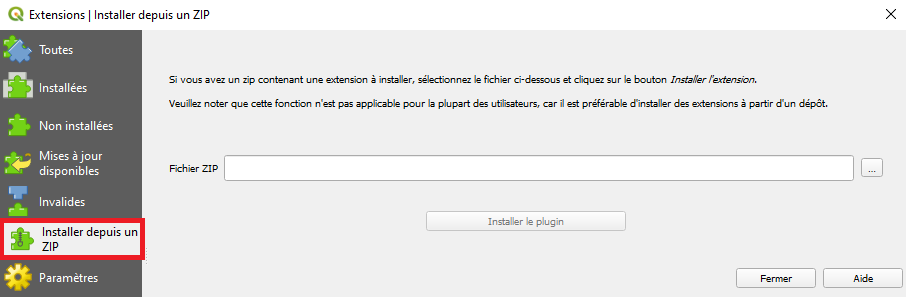
\includegraphics[width=1\linewidth]{1_installation_requirements/fig/QGIS_install_from_zip.png}
    \caption{QGIS dialog box for plugin management.}
    \label{fig-QGIS_install_from_zip}
\end{figure}

Once the \script{.zip} file has been extracted in QGIS, it may be necessary to activate it in the same plugin management window by navigating to the \gui{Installed} panel. The \cwv~extension must be checked to appear in the QGIS toolbar (\cref{fig-CWV-activation}).

\begin{figure}[H]
    \centering
    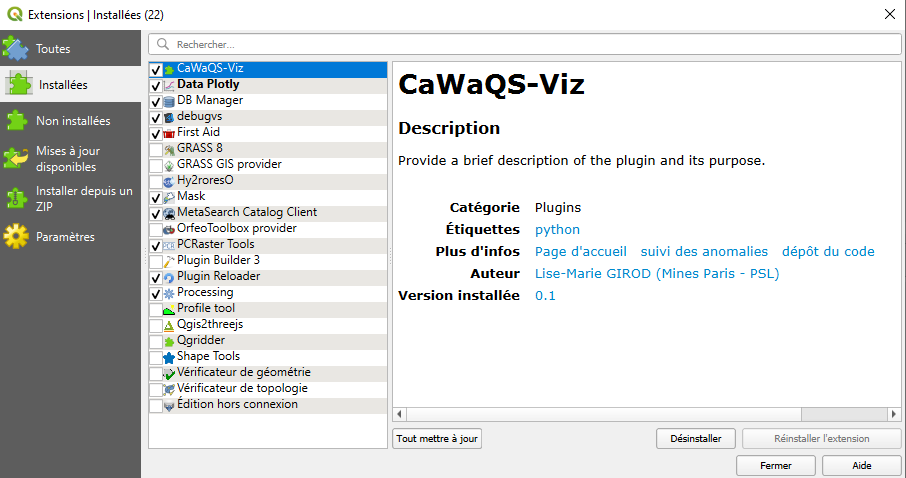
\includegraphics[width=1\linewidth]{couverture/fig/QGIS_get_plugin_in_toolbar.png}
    \caption{Activating the \cwv~extension in the QGIS application.}
    \label{fig-CWV-activation}
\end{figure}

Once the application is present in the QGIS toolbar, it is ready to be launched with a single click on the icon 
\includegraphics[height=0.45cm]{couverture/fig/Icon_CaWaQSVIZ.png}.

\subsection{What happens on first launch} \label{sec-install-bootstrap}

On the first launch after a ZIP installation, the plug-in automatically runs \script{pip install --user --upgrade external/HydrologicalTwinAlphaSeries} to register the backend and resolve its Python dependencies. This requires an internet connection and lands in your per-user site-packages (\script{\textasciitilde/.local/lib/pythonX.Y/site-packages} on Linux, \script{\%APPDATA\%\textbackslash Python\textbackslash...} on Windows). Subsequent launches are no-ops.

On Debian/Ubuntu and derivatives that ship a PEP~668 ``externally-managed'' system Python, the plug-in automatically retries with \script{--break-system-packages} (the install still lands in your per-user site-packages, not in apt-managed system paths).

If the install fails, the QGIS Python console prints the exact \script{pip} command you can run manually to diagnose.

\alertinfo{To use any new update of the plug-in installed via ZIP, it will be necessary to repeat this entire procedure (\cref{sec-install-user}). With Option 1, updating is done with \script{git pull} instead (\cref{sec-install-pixi-update}).}

\section{Dependency Installation} \label{setup-dependances}

Dependencies are handled automatically. With Option 1, \script{pixi} pins and installs QGIS, Python, and every dependency inside the project folder (\cref{sec-install-pixi}). With Option 2, the first-launch bootstrap resolves the backend and its Python dependencies (\cref{sec-install-bootstrap}). No manual dependency installation is normally required.

\alertinfo{If the first-launch bootstrap fails, the QGIS Python console prints the exact \script{pip} command to run. As a fallback, dependencies can still be installed manually from the Python interpreter built into QGIS. Installing them from any other interpreter will not allow QGIS to access the required libraries.}

The core Python dependencies are: \script{pandas}, \script{numpy}, \script{ipython}, \script{matplotlib}, and \script{geopandas}. As a manual fallback, open a QGIS Python console\footnote{By clicking on 
\includegraphics[height=0.45cm]{1_installation_requirements/fig/interpreteur_python.png} in the QGIS interface.} and run:

\begin{lstlisting}[language=python]
>>> import pip
>>> pip.main(['install', 'pandas', 'numpy', 'ipython', 'matplotlib', 'geopandas'])
\end{lstlisting}

\section{Developer Installation} \label{sec-install-expert}

For development purposes, and to make it easier to update the plug-in from the QGIS interface, the plug-in can be installed directly in the QGIS \emph{native} extensions directory. The \gitlab~repository for \cwv~can be cloned from a command terminal, remembering to initialise the backend submodule:

\begin{lstlisting}[language=bash]
$ git clone https://gitlab.com/gviz/cawaqsviz
$ cd cawaqsviz
$ git submodule update --init external/HydrologicalTwinAlphaSeries
\end{lstlisting}

The application directory must be placed at the location (folder) of the native QGIS applications so that any modification of the plug-in source code can be taken into account by QGIS at startup. The QGIS directory is accessible \textit{via} the following path:

\begin{lstlisting}[language=bash]
#windows
C:/Programmes/QGIS3.X.X.X/apps/qgis-ltr/python/plugins/
#linux
~/.local/share/QGIS/QGIS3/profiles/default/python/plugins/
\end{lstlisting}


The plug-in code structure is described in chapter \ref{chap-description-src}.\\

\alertinfo{Autocompletion of features related to the qgis library is available provided the Python interpreter used by QGIS is used. A virtual environment can be initialised for this purpose.}

\textbf{N.B.}: To facilitate plug-in development, the following utilities can be installed from the QGIS application manager:
\begin{enumerate}
    \item \textbf{Reloader} allows reloading the plug-in without restarting QGIS after each code modification,
    \item \textbf{FirstAid} provides a detailed view of errors returned by the QGIS Python interpreter as well as the various objects and variables related to the extension.
\end{enumerate}
